Bij het kijken naar figuur \ref{fig:tijd} valt meteen op dat \textit{Fast Non-Local Mean Denoising} niet efficiënt is. Dit resultaat ligt binnen de verwachtingen door de manier waarop deze methode te werk gaat, zie sectie \ref{subsec:fnlmd}. De waarde blijft nagenoeg constant doordat deze methode geen kernelgrootte heeft, hij is trager met grootteorde drie ten opzichte van de andere filters. Om deze reden zal deze filter niet opgenomen worden in het project. 

\begin{figure}[h!]
    \centering
    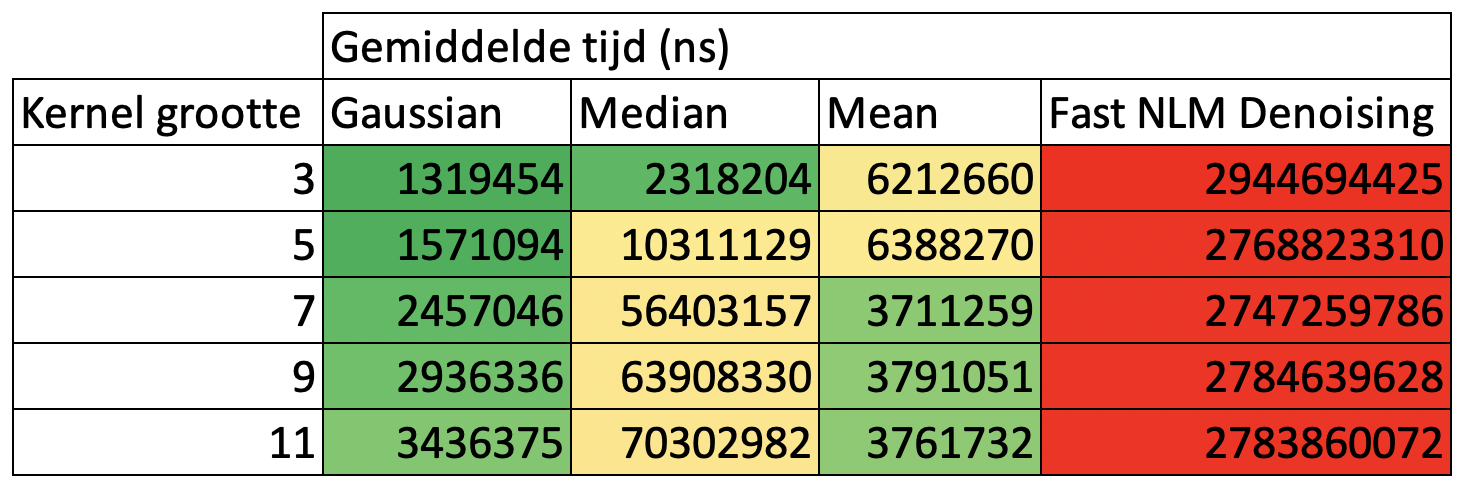
\includegraphics[width=\linewidth]{img/tijdsconsumptie}
    \caption{Gemiddelde tijd nodig om filter op afbeelding toe te passen.}
    \label{fig:tijd}
\end{figure}

Voor de andere filters kunnen hun individuele tijdsgrafieken, zie figuur \ref{fig:tijdsgrafieken}, van dichterbij bekeken worden. 
Bij het bekijken van deze tijdsgrafieken, is bij de \textit{Gaussian filter} een duidelijk lineair verband tussen zijn kerngrootte en de tijdsconsumptie zichtbaar. Dit wordt bevestigd door de determinatiecoëfficiënt van 97,85 procent van de lineaire trendlijn. 

\paragraph{}
Verder zijn er nog twee opvallende zaken; enerzijds zorgt een grotere kern ervoor dat de \textit{Median filter} veel meer tijd nodig heeft. De reden hiervoor is dat hoe groter de kern, hoe meer elementen pixelwaarden gesorteerd moeten worden van klein naar groot. Bij de {\it Mean filter} zou het zelfde gedrag verwacht worden. Rond kerngrootte zeven is er echter een sprong, de verklaring hiervoor is niet gevonden en eist verder onderzoek.

 \begin{figure}[h!]
  \centering
  \begin{subfigure}{0.4\linewidth}
    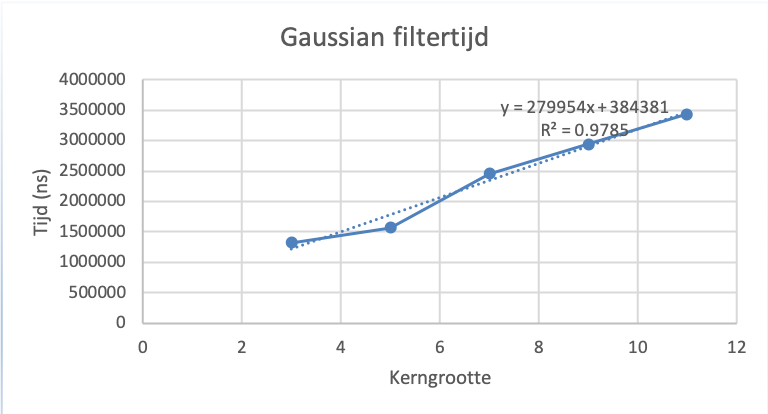
\includegraphics[width=\linewidth]{img/gaussiantijd}
  \end{subfigure}
  \begin{subfigure}{0.4\linewidth}
    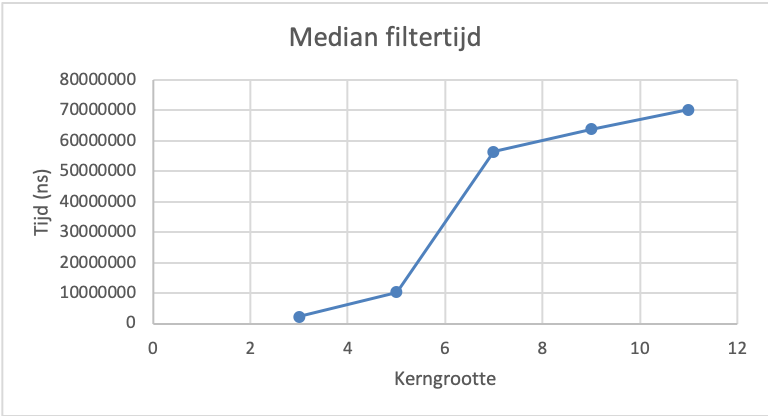
\includegraphics[width=\linewidth]{img/mediantijd}
  \end{subfigure}
  \begin{subfigure}{0.4\linewidth}
    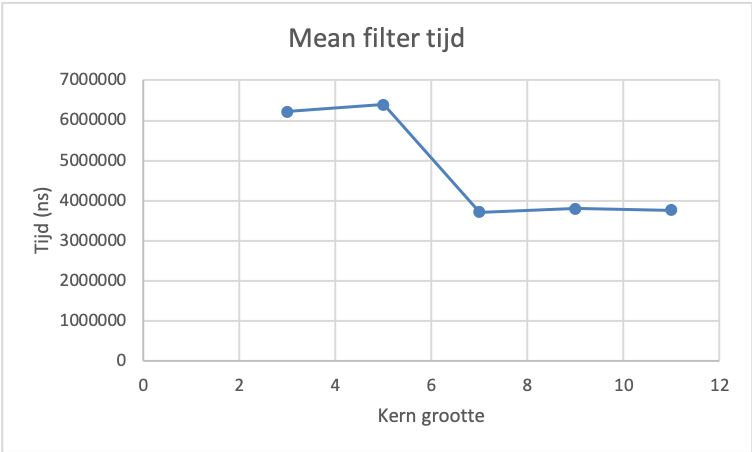
\includegraphics[width=\linewidth]{img/meantijd}
  \end{subfigure}
  \caption{Tijdsgrafieken voor de verschillende filters}
  \label{fig:tijdsgrafieken}
\end{figure}

{\it Gaussian} en {\it Medain blur} geven de beste resultaten, gekeken naar de tijdscomponent.  De \textit{Fast Non-Local Mean Denoising} is door dezelfde component afgeschreven.



